\subparagraph*{Submission : }
\textit{Consider the case in which the assignment of promos is fixed and the price of the second itm is fixed and the goal is to learn the optimal price of the first item. Assume that the number of users per class is known as well as the conversion rate associated with the second item. Also assume that the prices are the same for all: the classes (assume the same in the following) and that the conversion rates do not change unless specified differently below. Adopt both an upper-confidence bound approach and a Thompson-sampling approach and compare their performance.}\\

The request is to learn the optimal price of the first item, comparing the adoption of a Thompson-sampling approach and an Upper-Confidence Bound approach

\subsection*{Basic knowledge}
The described problem is a combinatorial bandit problem, which is a decision making problem in where decision maker selects one single arm in each round, and observes a realization of the corresponding unknown reward distribution. Each decision is based on past observed rewards. The objective is to maximize the expected cumulative reward over some time horizon by balancing exploitation and exploration. We can solve it, through an online algorithm, where only for the feasible solutions we will have precise estimations. Thomspon-Sampling algorithm (TS) and Upper-Confidence Bound algorithm (UCB1) are well known algorithm used to solve combinatorial bandits problem.

\subparagraph*{Upper-Confidence Bound (UCB1)}

\begin{itemize}
	\item Every arm is associated with an upper confidence bound 
	\item At every round, the arm with the highest upper confidence bound is chosen
	\item After having observed the realization of the reward of the arm, the upper confidence bound is updated
\end{itemize}
Notation:\\
\begin{itemize}
\item $t$ time
\item $A$ set of arms
\item $a$ arm
\item $a_{t}$ arm played at time $t$
\item $a^*$ optimal arm
\item $X_{a}$ random variable (bernoulli) associated to arm a
\item $\mu_{a}$ expected value of random variable $X_{a}$
\item $x_{a,t}$ realization of random variable $X_{a}$ at time $t$
\item $x_{a}$ realizations of $X_{a}$
\item $\bar{x}_{a}$ empirical mean of $x_{a}$
\item $n_{a}(t)$ number of samples of arm $a$ at time $t$
\end{itemize}

Pseudocode\\

1. Play once each arm $a \in A$

2. At every time $t$ play arm $a$ such that:

\hspace{2em}$a_{t} \leftarrow \argmax_a{\left\{\left[\bar{x}_{a} + \sqrt{\frac{2 log(t)}{{n_{a}(t-1)}} }\right]\times a\right\}}$

\subparagraph*{Thompson Sampling (TS)}

\begin{itemize}
	\item For every arm, we have a prior on its expected value 
	\item In the case the arms’ rewards are Bernoulli distribution, the priors are Beta distributions
	\item Notice that, with the opportune parameters, a Beta distribution is a uniform distribution 
	\item For every arm, we draw a sample according to the corresponding Beta
	\item We choose the arm with the best sample 
	\item We update the Beta distribution of the chosen arm according the observed realization
\end{itemize}

Notation (in addition to classical UCB):\\
\begin{itemize}
	\item $\mathbb P(\mu_{a}=\theta_{a})$ prior of the expected value of $X_{a}$
	\item $\theta_{a}$ variable of $\mathbb P(\mu_{a}=\theta_{a})$
	\item $(\alpha_{a_{t}}, \beta_{a_{t}})$ parameters of the beta distribution $P(\mu_{a}=\theta_{a})$
\end{itemize}

Pseudocode\\

1. At every time $t$ for every arm $a$:

\hspace{2em}$\tilde{\theta_{a}} \leftarrow Sample(\mathbb P(\mu_{a}=\theta_{a}))$ \\

2. At every time $t$ play arm $a_{t}$ such that 

\hspace{2em}$a_{t} \leftarrow \argmax_a \left\{ \tilde{\theta_{a}} \times a \right\} $ \\

3.  Update beta distribution of arm $a_{t}$

\hspace{2em}$(\alpha_{a_{t}}, \beta_{a_{t}}) \leftarrow (\alpha_{a_{t}}, \beta_{a_{t}}) + (x_{a_{t},t}, 1 - x_{a_{t},t})$


\subsection*{Strategy}

In our solution we simulate a random arrival of the customers, through two different leaners, TS learner and a UCB learner, we extract from our candidates two prices and we emulate the purchase phase using both prices. In case the customer buys the first item, we propose the second one at a fixed price, computed according to the customer category. In this case we do not simulate the purchase phase, but we use the knowledge of the conversion rate of the second item to compute the final customer reward. 

\subparagraph{Implementation} 
\begin{itemize}
	\item No seasonality, conversion rate do no change
	\item Number of customers per class is known 
	\item Candidates for the \textit{Racing Skis} are: \{2260.0,1910.0,2130.0, 2010.0, 2340.0\}
	\item Conversion rate associated with the first item is not known
	\item Basic price of the Racing Ski Helmet is fixed to 630.0
	\item Promotion assignment is fixed, according to the results of our offline solution: 
	\begin{center}
		\begin{tabular}{ |c|c|c|} 
		\hline
		User category & Assigned promotion & Racing Ski Helmet price \\
		\hline
		Sport Addicted & P$_2$ : 20\% & 504.0 \\
		\hline
		Gifter & P$_1$ : 10\% & 567.0 \\
		\hline
		Amateur & P$_0$ : 0\% & 630.0 \\
		\hline
		Worried & P$_3$ : 30\% & 441.0 \\
		\hline
		\end{tabular}
	\end{center}
	\item Conversion rate associated with the second item is known
\end{itemize}

Both UCB and TS learner expect as learnign parameter a binomial value, while our reward is value composed by the sold of the first item plus the eventual sold of the second item. In order to normilize the reward to be passed learner, we divide the customer reward by the maximum achievable reward.   

\subparagraph{Optimal strategy}In order to compute a regret, the simulated rewards are compared with an optimal solution that, accordingly to the conversion rates for the first items, is to offer the \textit{Racing Skis} at the lower price (1910.0 according to our candidates prices). 

\subsection*{Results}
\begin{center}
	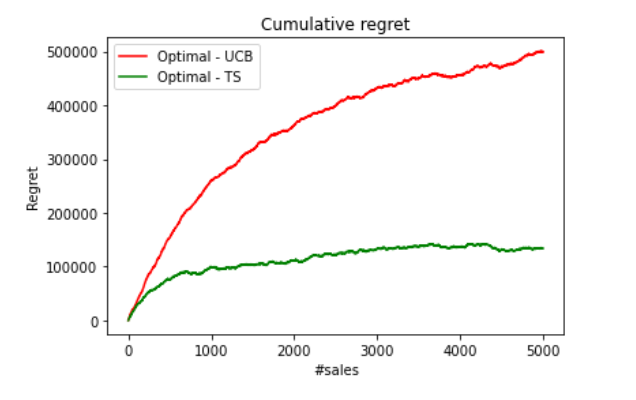
\includegraphics[scale=1.2]{Images/n3}
\end{center}
Days: 10\\
Experiments number: 10 \\
Both UCB and TS strategy converge on 1910.0\\
\textit{We decide to plot the regret of the first 5000 clients, since plotting the results of the entire time horizon made the plot unreadable}


\subsection*{Considerations}
As we can observe in the plot, both approach converge to a stable solution, however Thompson Sampling approach performs better than a UCB approach. Infact Thompson Sampling is faster to find the best price for the first item than UCB and this allow to have a lower regret. 